%---
%From the draft paper

%Charge exchange collisions cause neutral atoms to donate an electron to thermal ions thereby creating a hot neutral and a cold ion, representing a transfer of ion heat to the neutral population. In PPCD plasmas where other loss mechanism are reduced, charge exchange becomes a dominant heat transfer process.  In previous estimates, the neutral fluid is assumed to be cold, therefore, exchange collisions tends to equlibrate ions with this "cold" neutral fluid. This assumption is incorrect. The mean free path of a "cold" neutral is very short (<1cm)[[Recheck this]], but edge neutrals may undergo subsequent charge exchange collisions resulting in higher temperature neutrals that can penetrate into the plasma Consequently, neutrals in the core are mostly generated near the mid-radius and have a temperature comparable to mid-radius ions. At the same time, a charge exchange neutral created from thermal neutral in the core, if traveling through core-like conditions, has a mean free path shorter than the minor radius, implying a fraction of such neutrals would undergo secondary ionization or charge exchange reactions. Since neutral-neutral collisions are rare($Kn \simeq 0.8$), the hot neutral species cannot be adequately treated as a fluid and have to be treated with a kinetic model. 

%$D_{\alpha}$ emission is dominated by emission in the plasma edge where neutral density is high. As the core contributes negligible emissions, a simple inversion of line integrated measurements has difficulty capturing anything more detailed than an upper bound of the core neutral density. Therefore, physics-based equilibrium modeling is needed to construct self-consistent core neutral profiles that produce the observed $D_{\alpha}$ emissions. There was a previous attempt to use a Monte Carlo simulation, constrained by $D_\alpha$ emissions,  to determine neutral density\cite{Eilerman2012Time-resolvedPinch}, but it relied on a spatially uniform \textit{ad hoc} neutral particle source at 50eV in addition to wall sources to fit the observations. This model's ability to fit PPCD measurements was poor compared to standard RFP discharges. Additionally, previous work using neutral density as part of impurity charge state balance calculations found that the core neutral density was likely over-predicted\cite{Barbui2014,Kumar2012a}.

%\begin{figure*}
%	\centering
%	\includegraphics[width = 0.9\linewidth]{./neutral_triple_plot_alt.png}
%	\caption{Neutral analysis results. A). Typical neutral density result from DEGAS2 show a rapid drop off towards the core. There are two notable asymmetries: the Shafranov shift result in lower neutral density on the outboard side, and the gas puffing prior to the PPCD period leaves a residual up/down asymmetry. The dotted lines mark out the sight-lines of the detector array, and the different colored borders mark the three source locations. B) Neutral modeling results also show a corresponding `rise' in temperature as one moves towards the core. This produces a charge exchange loss profile that is both lower and more hollow than estimates assuming cold neutrals. C). Flux surface averaged $P_{CX}$ at 13ms, showing significantly hollowing of the loss term.}\label{fig:neutral_triple}
%\end{figure*}%

%For this work, DEGAS2, a 2-D Monte Carlo simulation that produces neutral density and temperature profiles\cite{StotlerDEGAS2Manual}, is used to model core neutral profiles. DEGAS2 takes $ T_{e} $ and $ n_{e} $ profiles as input and it tracks and tallies charge exchange, ionization, recombination, and molecular disassociation reactions, as well as associated particle and heat flow of test particles. Synthetic $ D_{\alpha} $ radiance measurements are created within DEGAS2 which are used to fit experimental measurements by varying boundary source rates as fitting parameters. Since the typical operation of PPCD plasmas entail no active gas puff fueling, all particle sources are related to recycling and pumping mechanisms. A three surface source geometry, each having an independent source rate is used, consisting of an outboard limiter, a pumping duct region (bottom 45\textdegree) and the rest of the wall (see Fig \ref{fig:neutral_triple} A). The outboard limiter is singled out for special attention due to the Shafranov shift causing the last closed flux surface to strike the outboard limiter rather than the inboard. Treating the pumping duct as a separate source is necessary to improve the fit quality in PPCD conditions. The sources and their contributions to the plasma are assumed to be linearly independent as neutral-neutral interaction is negligible. An example of the result of the DEGAS2 simulation at a single time point is shown in Fig~\ref{fig:neutral_triple}.

%\begin{figure}
%	\centering
%	\includegraphics[width = 1.\linewidth]{./plots/degas_neutral_t}
%	\caption{Neutral modeling results also show a corresponding `rise' in temperature as one moves towards the core. This produces a charge exchange loss profile that is both lower and more hollow than estimates assuming cold neutrals.}\label{fig:temp}
%\end{figure}

%EGAS2 simulations are evaluated at 0.5ms intervals due to both the computational cost of the Monte Carlo simulations, and the frequency at which $ T_e $ measurements, a key input, are available via TS. For the ensemble being analyzed, the typical reduced $\chi^2$ value of the fit to the measured $D_\alpha$ signal is ~0.6. The 2-D results are incorporated into the 1-D ion thermal model through flux surface averaging. DEGAS2 modeling shows $\frac{T_{neutral}}{T_{i}} \simeq 0.7$ in the core which, combined with lower $ n_{neutral} $, leads to lower charge exchange heat loss than previous estimates. Further, the charge exchange loss is found have a hollow profile (see Fig. \ref{fig:dedt_plot}), and is at a level that is broadly consistent with the temperature evolution of the ions without having to invoke additional anomalous heating terms during PPCD periods\cite{Fiksel2006}. 

%--end from paper

\section{Neutral dynamics in improved confinement MST plasmas}\label{sec:neutral_results}

The neutral dynamics are perhaps the most important factor in ion thermal transport in MST. This is not only through the direct consequences as those laid out in section \ref{sec:neutral_physics}, but due to it's effect on determining other effects mentioned in the following sections. As explain in previous sections in detail, the neutral dynamics can be difficult to measure directly, and physics modeling is needed. The inadequacy of inversion techniques and the need for physics simulation regarding neutrals is known previous\cite{Eilerman2012}, and there have been a previous attempt to model the neutrals using a Monte-Carlo simulation code called NENE \cite{NENE}. NENE is similar to the DEGAS2 code that is used for this modeling work. However, comparatively NENE did poorly for PPCD plasmas, and needed an \textit{ad hoc} 50eV uniform neutral source to improve the quality of fit\cite{Eilerman}. Further, the implementation of NENE on MST did not produce neutral temperature information, or the thermal effects of impact ionization, the importance of which becomes clear later in the section. The general setup of the neutral simulation with in the model has been laid out previously in section \ref{sec:DEGAS2}, but before the density and temperature results can be discussed, we need to have a short detour to talk about fitting quality and the source geometry used to obtain the fits.

\begin{figure}
	\centering
	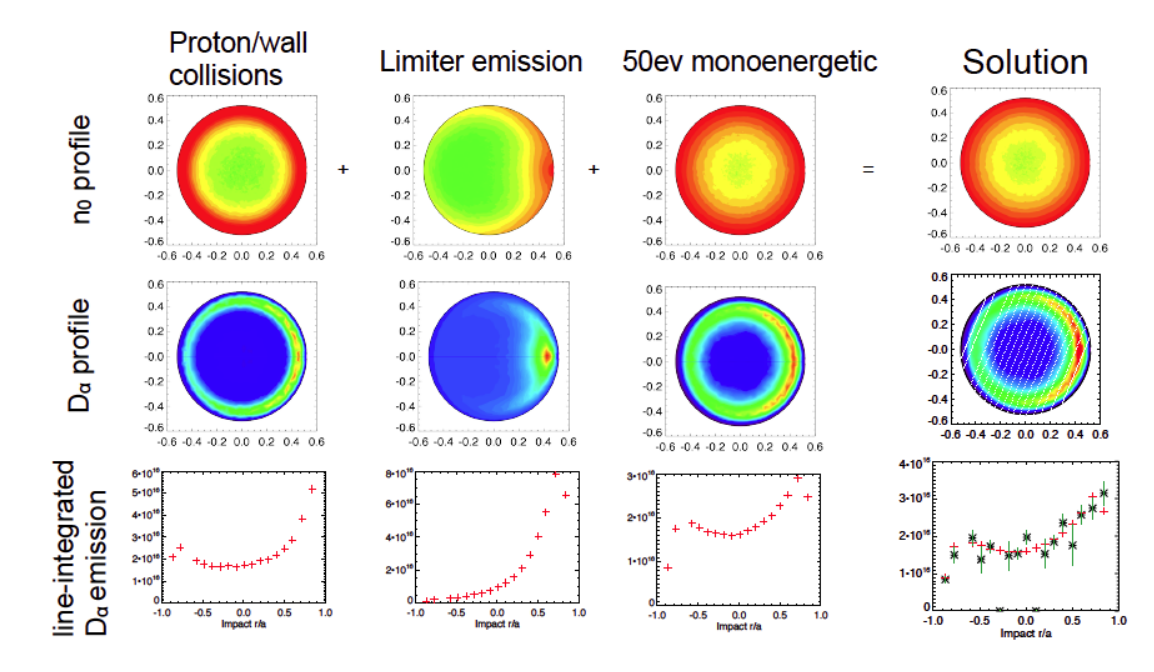
\includegraphics[width = 1.\linewidth]{ion_transport_results/nene_example.png}
	\caption[Example of NENE neutral output]{Example of NENE neutral output, the difference between this and the DEGAS2 results are examined in this section. (Reproduced from S. Eilerman's Thesis \cite{Eilerman})}\label{fig:nene_example}
\end{figure}

\subsection{Neutral source geometry, and fitting of observations}\label{sec:neutral_source_geometry}

In an ideal situation the neutral source rates would be known through direct observation and include all individual asymmetries. But as a practical matter, neutral recycling is complex and not in the scope of this work. Instead, the neutral simulation is run with several independent neutral source profiles. Each 'source' would have a certain defined geometry, and rate (which are uniform across the defined geometry). Each instance of neutral analysis would simulate the three sources independently, and then the rates are linearly fit to the observed $\dal$ emission levels (discussed in detail in section \ref{sec:DEGAS2}). Increasing the number of independent 'sources' via subdividing the wall geometry give more fitting parameters, but it makes the fitting problem (relatively) under constrained, and increases the computing power needed. This work uses a three-source geometry as follows (illustrated in figure \ref{fig:DEGAS2_sources_and_density}):
\begin{figure}
	\centering
	\includegraphics[width = 0.7\linewidth]{ion_transport_results/source_contrib.png}
	\caption{Geometry of the contributions of the 3 sources used in DEGAS2. It is interesting to point out that in the contribution from the 'uniform' source, there can be clearly observed the effect of the Shafronov shift on the neutral density. \textit{ie.} the neutral density 'hole' is correspondingly shifted to reflect the shift in the ionization region. This phenomenon is not seen in NENE results of the same source (figure \ref{fig:nene_example}), and it is unclear why. Though likely related to self-consistency issues in implementation.}\label{fig:DEGAS2_sources_contrib}
\end{figure}
\begin{enumerate}
    \item A poloidally localized source corresponding to the location of the outboard limiter. The outboard limiter (typically) defines the LCFS on MST and is known to be a major source of recycling as well as impurities.  
    \item A poloidally uniform source representing the walls of MST, with the exception of the area detailed in the following source. 
    \item A poloidally localized source corresponding to the bottom 45\textdegree of the wall. This is the location of the pumping and fueling duct of MST. 
\end{enumerate}
The contributions from each source (to density, for example) are treated as linearly independent. This is due to the fact that neutral, neutral interactions are very low compared to other physics at typical parameters. Typical contributions from each source are shown in figure \ref{fig:DEGAS2_sources_contrib} This project began by considering only the first two sources, with the second extending uniformly around the whole 'circle' of the vessel. However, it is found that on some shots, and some times during other shots, such a geometry would not quite be sufficient to explain the observation. In particular, the intensity on the central view chords would be systematically under-predicted by the code. By hypothesizing that the pumping duct, which is a separate non-plasma volume of the vacuum vessel below the plasma volume via which pumping and puff fueling are done, have a different source rate than 'the rest of the wall', the code is then able to give a much better fit to the observations (see figure \ref{fig:DEGAS2_2_3_source_comp}, and \ref{fig:DEGAS2_typical_fit}). Additionally, it is useful to point out that
\begin{figure}
	\centering
	\includegraphics[width = 0.7\linewidth]{ion_transport_results/2_3_source_comparison.png}
	\caption[Comparison between 2 source and 3 source fit for DEGAS2]{Comparison between 2 source and 3 source fit for DEGAS2.}\label{fig:DEGAS2_2_3_source_comp}
\end{figure}

\begin{figure}
    \centering
    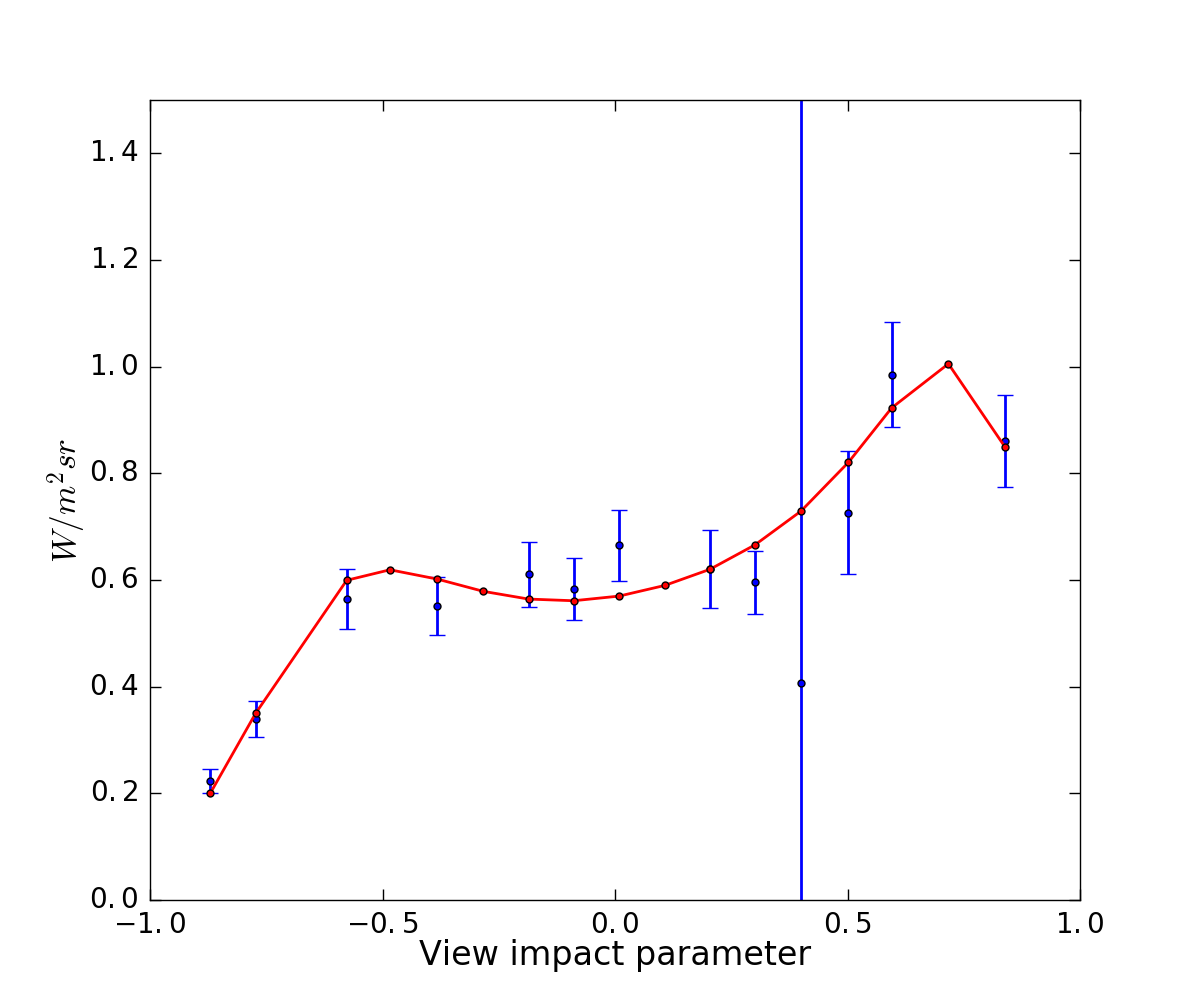
\includegraphics{ion_transport_results/DEGAS2_typical_fit.png}
    \caption{A typical DEGAS2 fit of ensembled $\dal$ signal.}
    \label{fig:DEGAS2_typical_fit}
\end{figure}

\subsection{Neutral density in PPCD}

\begin{figure}
    \centering
    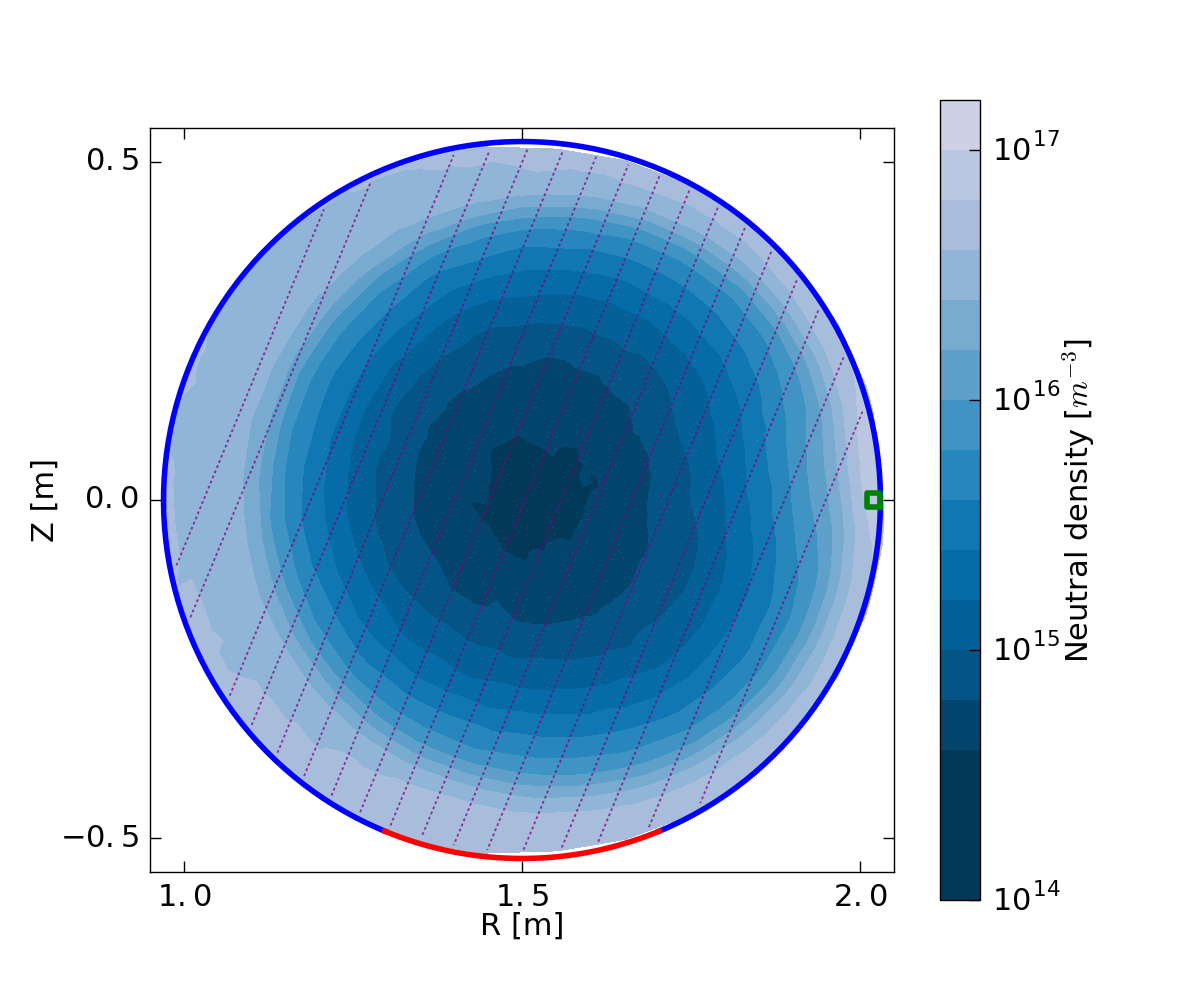
\includegraphics{ion_transport_results/DEGAS2_density2d.png}
    \caption[Neutral density via DEGAS2]{Neutral density via DEGAS2 simulation, with the geometry of the three sources overlayed. Using the numbering presented in section \ref{sec:neutral_source_geometry}: source 1 is in green, source 2 is in blue, and source 3 is in red. }
    \label{fig:DEGAS2_sources_and_density}
\end{figure}


Unsurprisingly, the neutral density is edge dominated and decreases by about 2.5 orders of magnitudes as one 'travels' towards the core. The details can be seen in figure \ref{fig:DEGAS2_sources_and_density} and \ref{fug:DEGAS2_1d}. The edge neutral density is comparable with previous estimates, and the core density is ~1/4 from NENE estimates presented by S. Eilerman at APS-DPP\cite{Eilerman2010}. Though when NENE is run for my particular shot ensemble, it returns results lower than that presented, and the core density from DEGAS2 is ~ 55\% of NENE. As pointed out above, the DEGAS2 fit have the advantage of not relying on an \textit{ad hoc} 50eV neutral source to achieve the fit, and the neutral density more self consistently show the effect of the Shafronov shift (see also figure \ref{fig:DEGAS2_sources_contrib}). Further, the neutral density in PPCD is not entirely constant; the early part of PPCD sees the neutral density decreasing until around 16.5ms when it stabilizes until the end of PPCD (figure \ref{fig:neutral_vs_time}. This neutral density estimates is also in line with that from s. Kumar's measurement of Al charge state fractions in the core. The charge state fraction of Al$^{11+}$ to Al$^{13+}$ is very sensitive to neutral density as the charge exchange process keep the Al$^{13+}$ population down. DEGAS2's estimate of core neutral density. The DEGAS2 neutral density is still too might to match that needed by J. Waksman to explain the NBI heating effects observed. However, this is perhaps not a good direct comparison as his work are on well optimized low current (200kA) PPCD, which, other than the problem of differing plasma current as my parameters, is inherently difficult for $\dal$ observations to constrain neutral density as the emission measurements begin to approach noise levels of the detector. 

\begin{figure}
    \centering
    \includegraphics{ion_transport_results/DEGAS2_temperature_1d2d.png}
    \caption[Neutral temperature via DEGAS2]{Neutral temperature via DEGAS2 simulation. A) The 2-d temperature results. B) The flux surface averaged results, with $T_i$ for comparison. and C) the neutral temperature ratio $\equiv \frac{T_{D^0}}{T_D}$.}
    \label{fig:DEGAS2_temperature}
\end{figure}

Another notable improvement of the understanding of the neutral dynamics is the neutral temperature information provided by DEGAS2. Though it may not be immediately obvious, but a high $T_{\text{neutral}}$ is needed for the neutrals to penetrate into the plasma volume. The mean free path of a 'room temperature' neutral is very short in MST parameters, and neutrals created by charge exchange reactions, and a small amount of Frank-Condon neutrals from energetic disassociation of D$_2$ would dominate the neutrals interior to the plasma. This is reflected by the DEGAS2 results (figure \ref{fig:DEGAS2_temperature}). Notably, the neutral temperature is a significant fraction of the ion temperature, meaning that only a fraction of the ion's thermal energy is effectively lost in a charge exchange reaction.

\subsection{Charge exchange, impact ionization, and ion source rate}

\begin{figure}
    \centering
    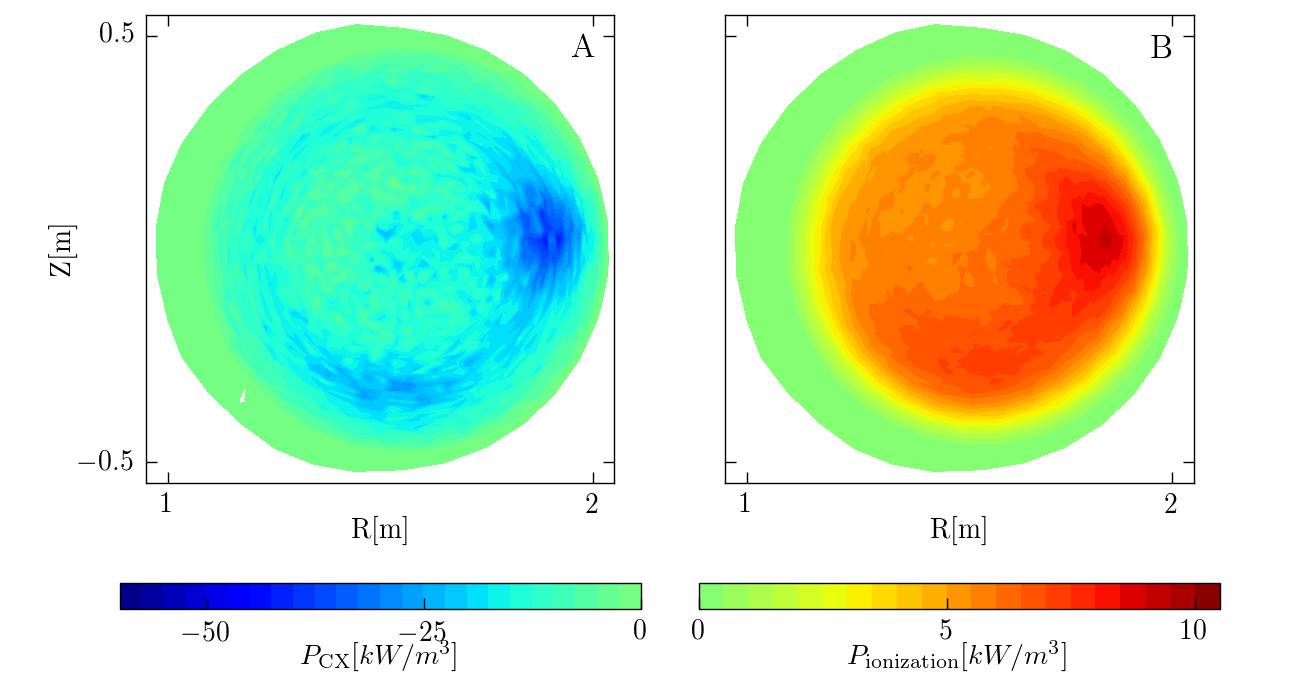
\includegraphics{ion_transport_results/DEGAS2_power_terms_2d.png}
    \caption{DEGAS2 2D charge exchange (a) and impact ionization (b) terms.}
    \label{fig:DEGAS2_power_2d}
\end{figure}

\begin{figure}
    \centering
    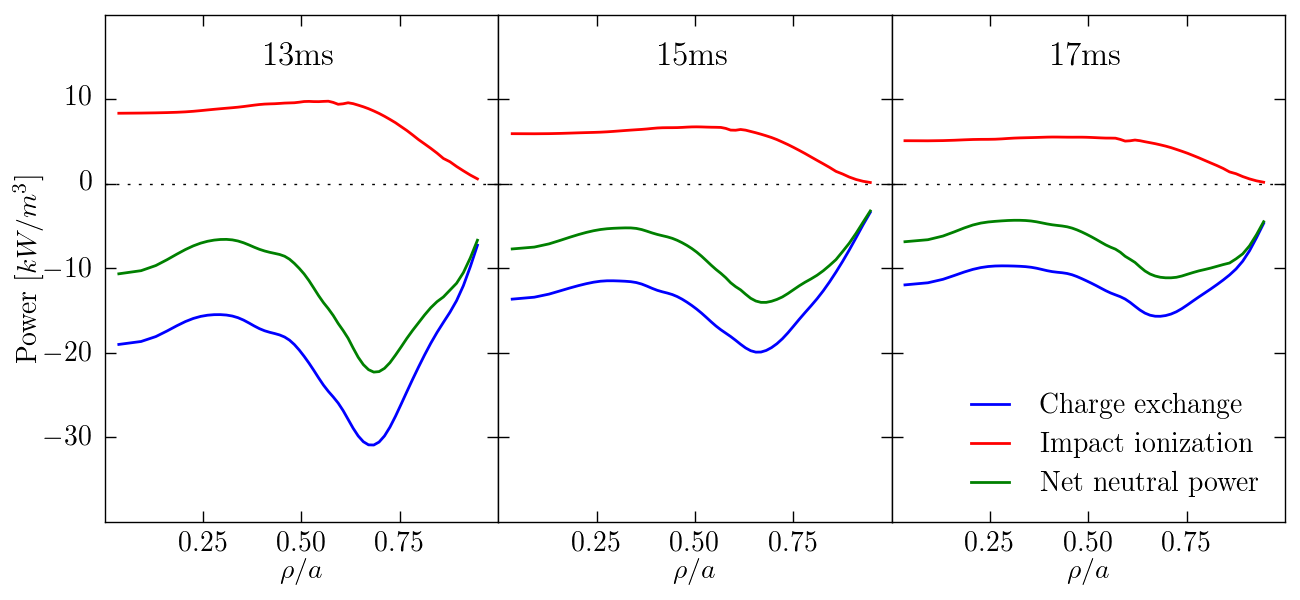
\includegraphics{ion_transport_results/DEGAS2_power_terms_1d.png}
    \caption{1-D neutral power terms at 13ms, 15ms, and 17ms. The 'net charge exchange loss' refers to the sum of the two terms, as electron impact heating is a process that recovers some thermal energy from the neutrals fuild.}
    %This plot should include 'net charge exchange loss'
    \label{fig:DEGAS2_power_1d}
\end{figure}


The charge exchange loss rate displays an hollow profile that is significantly skewed outboard, like the ion density. However, the poloidal transit time are small on the RFP and neutral effect on the majority ion fluid is still considered on a flux surface averaged basis despite significant asymmetry. On a practical basis, this hollow profile is the creation of the declining neutral density towards the core, and the increasing majority density as well as temperature difference. The trend of declining neutral density also translates to the charge exchange loss as expected. The electron impact heating is an interesting to consider as it represents a partial 'recovery' of the thermal energy lost in charge exchange (details in section \ref{sec:neutral_physics}). However, as the neutral's temperature is below that of majority ion, this actually results in temperature decrease. In general, I use 'heating' to describe thermal energy input into the ion fluid which does not necessarily increase the temperature. 

\begin{figure}
    \centering
    \includegraphics{ion_transport_results/DEGAS2_source_rate.png}
    \caption{DEGAS2 ion source rate results.}
    \label{fig:DEGAS2_power_1d}
\end{figure}

The ion source rate also displays the same characteristics as the power terms. However, it is significantly more hollowed out since it does not depend on the difference in ion and neutral temperature, which is higher in the core. This means that the ion source rate is not sufficient to explain the density rise in the core. The consequence of this is to hint at an inward pinch mechanism to be explained in more detail in section \ref{sec:eb_pinch}

\subsection{Unintuitive model response of \textit{ad hoc} heating in the edge}
\begin{figure}
    \centering
    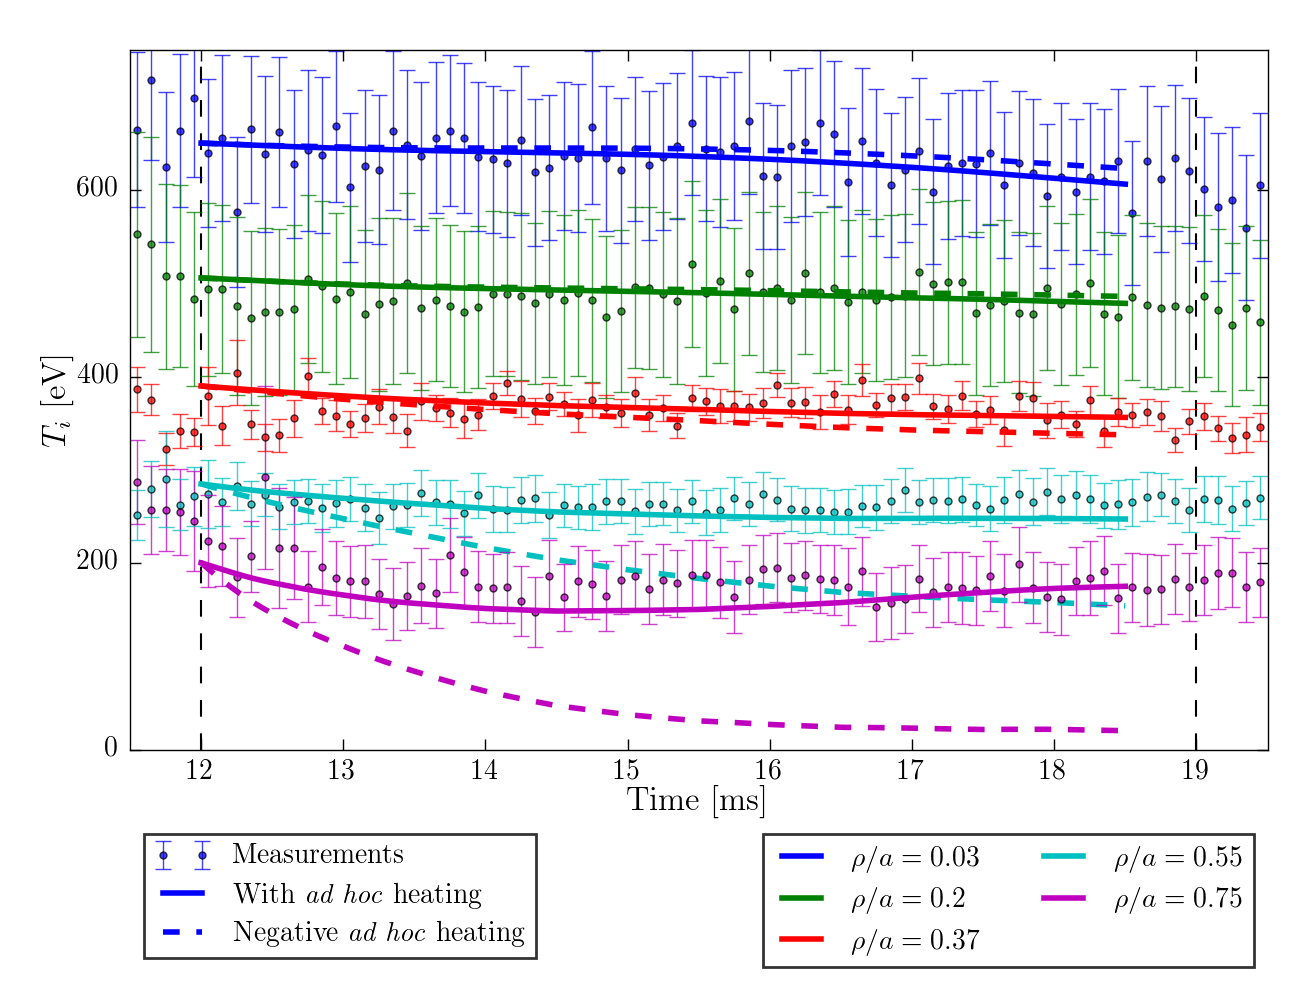
\includegraphics{ion_transport_results/unintuitive_response.png}
    \caption{The effect of having a low ion temperature edge on charge exchange}
    \label{fig:unintuitive_cx_response}
\end{figure}

During this project, and the adjustment process for the model, it became clear that ion heating in the edge have an effect on the charge exchange loss in the core through it's effect on ion temperature. Suppose you have an edge region where the ion temperature is only a few eVs, but the electrons are on the order of 50 to 100 eV. In this region, electron impact ionization of neutrals would dominate charge exchange, and any neutral particle entering the plasma would more likely be ionized before undergoing charge exchange, thus decreasing the neutral penetration. The decreased penetration would in turns result in a more hollowed out neutral density, as well as charge exchange loss and ion source rate. This situation was created in the model from a mistake in the calculation in the flow effects in the edge, and when \textit{ad hoc} heating is applied this erroneous model to bring it inline with the observed temperature without changing how the rest of the model is calculated, the core temperature is predicted to be lower. However, this effect seems most significant when the edge ion temperature drops to ~10eV or lower for a significant radius. When the mistake was corrected, the model predicted edge ion temperature of ~50eV at $\rho_v/a \approx 0.75$ without \textit{ad hoc} heating terms, and increasing it to the observed ~175eV using \textit{ad hoc} heating only dropped the core temperature slightly.

